\documentclass[10pt,a4paper]{article}

% -----------------------------------------------------------------------------
% Relatorio final - Mini GPU SIMD
% Estrutura compacta planejada para aproximadamente 10--12 paginas.
% Revise todos os campos [PREENCHER] e as notas de consistencia antes da entrega.
% -----------------------------------------------------------------------------

\usepackage[utf8]{inputenc}
\usepackage[T1]{fontenc}
\usepackage[portuguese]{babel}
\usepackage{lmodern}
\usepackage{microtype}
\usepackage{geometry}
\usepackage{graphicx}
\usepackage{array}
\usepackage{booktabs}
\usepackage{longtable}
\usepackage{tabularx}
\usepackage{multirow}
\usepackage{float}
\usepackage[section]{placeins}
\usepackage[table]{xcolor}
\usepackage{enumitem}
\usepackage{pdflscape}
\usepackage{tikz}
\usepackage{hyperref}
\usepackage{fancyhdr}
\usepackage{caption}
\usepackage{amsmath}
\usepackage{url}
\usetikzlibrary{arrows.meta,positioning,fit}
\graphicspath{{docs/}{./}}

\geometry{top=1.8cm,bottom=1.8cm,left=2.0cm,right=2.0cm}
\setlength{\parindent}{1.0em}
\setlength{\parskip}{0.25em}
\setlength{\tabcolsep}{4pt}
\renewcommand{\arraystretch}{1.12}
\setlist{nosep,leftmargin=1.4em}
\captionsetup{font=small,labelfont=bf}
\renewcommand{\tablename}{Tabela}
\renewcommand{\figurename}{Figura}
\addto\captionsportuguese{\renewcommand{\contentsname}{Sumário}}
\newcolumntype{L}[1]{>{\raggedright\arraybackslash}p{#1}}
\newcolumntype{Y}{>{\raggedright\arraybackslash}X}

\definecolor{azul}{HTML}{1F4E78}
\definecolor{azulclaro}{HTML}{D9EAF7}
\definecolor{cinzaclaro}{HTML}{F2F2F2}
\definecolor{cinzaescuro}{HTML}{555555}
\definecolor{alerta}{HTML}{8A3B12}

\hypersetup{
  colorlinks=true,
  linkcolor=azul,
  urlcolor=azul,
  citecolor=azul,
  pdftitle={Desenvolvimento e Verificacao de uma Mini GPU SIMD},
  pdfauthor={Vinicius Carvalho Pimpim}
}
\urlstyle{tt}

\pagestyle{fancy}
\fancyhf{}
\lhead{Projeto Final -- CI Digital}
\rhead{Mini GPU SIMD}
\cfoot{\thepage}
\setlength{\headheight}{13pt}

\newcommand{\signal}[1]{\texttt{\detokenize{#1}}}
\newcommand{\todo}[1]{\textcolor{alerta}{\textbf{[PREENCHER: #1]}}}
\newcommand{\module}[1]{\texttt{#1}}
\newcommand{\req}[1]{\texttt{\detokenize{#1}}}

\title{\textbf{Desenvolvimento e Verificação de uma Mini GPU SIMD}}
\author{Vinícius Carvalho Pimpim\\Projeto Final -- CI Digital}
\date{[MÊS / ANO]}

\begin{document}

% =============================================================================
% CAPA (pagina 1)
% =============================================================================
\hypersetup{pageanchor=false}
\begin{titlepage}
  \centering
  {\large [NOME DA INSTITUIÇÃO]\\[0.25cm]
  [CURSO / DISCIPLINA]}\par
  \vspace{2.8cm}
  {\Huge\bfseries Desenvolvimento e Verificação de uma Mini GPU SIMD\par}
  \vspace{0.6cm}
  {\Large Relatório técnico -- Projeto Final de CI Digital\par}
  \vfill
  {\Large Vinícius Carvalho Pimpim\par}
  \vspace{0.4cm}
  {\large [DOCENTE / ORIENTADOR, SE APLICÁVEL]\par}
  \vfill
  {\large [CIDADE]\\[0.2cm][ANO]\par}
\end{titlepage}
\hypersetup{pageanchor=true}

% =============================================================================
% RESUMO E SUMARIO (pagina(s) 2--3, conforme a extensao)
% =============================================================================
\pagenumbering{roman}
\section*{Resumo}
Este trabalho apresenta o desenvolvimento e a verificação de uma unidade de processamento vetorial simplificada baseada no paradigma SIMD (\textit{Single Instruction, Multiple Data}). A arquitetura combina 4 unidades aritméticas de 16 bits em uma unidade de processamento central capaz de executar a mesma operação sobre elementos independentes de dois vetores.  O sistema inclui memória vetorial de acesso dual-port, interface de requisições por pacotes, decodificação de comandos, escalonamento e controle de execução por máquina de estados. A implementação RTL foi escrita em SystemVerilog e verificada por meio de simulação e testes direcionados a cada módulo bem como a criação de um ambiente UVM com \textit{scoreboard}, cobertura funcional e assertions. São apresentados resultados de síntese, análise temporal e simulações da netlist, incluindo uma execução com anotação SDF.

\noindent\textbf{Palavras-chave:} SIMD; GPU; SystemVerilog; UVM; verificação digital; análise temporal.

\vspace{0.5em}
\section*{Abstract}
\textit{This work presents the development and verification of a simplified vector processing unit based on the SIMD (Single Instruction, Multiple Data) paradigm. The architecture uses four 16-bit arithmetic units to apply the same operation to independent elements of two vectors. The system includes dual-port vector memory, a packet-based request interface, command decoding, scheduling, and finite-state-machine control. The design was described in SystemVerilog and verified using directed tests and a UVM environment with a scoreboard, functional coverage, and assertions. Synthesis, timing analysis, and gate-level simulation results, including SDF annotation, are also presented.}

\vspace{0.5em}
\section*{Lista de abreviações e siglas}
\begin{tabularx}{\textwidth}{@{}lY@{}}
ALU & \textit{Arithmetic Logic Unit} (unidade aritmética e lógica)\\
AXI & \textit{Advanced eXtensible Interface}\\
FSM & \textit{Finite State Machine} (máquina de estados finitos)\\
GPU & \textit{Graphics Processing Unit}\\
RTL & \textit{Register Transfer Level}\\
SDF & \textit{Standard Delay Format}\\
SIMD & \textit{Single Instruction, Multiple Data}\\
SVA & \textit{SystemVerilog Assertions}\\
UVM & \textit{Universal Verification Methodology}
\end{tabularx}

\clearpage
\tableofcontents

% Para economizar paginas, as listas de figuras e tabelas nao sao inseridas
% automaticamente. Caso sejam exigidas, descomente os comandos abaixo e reveja
% o limite total de paginas:
% \listoffigures
% \listoftables

\clearpage
\pagenumbering{arabic}

% =============================================================================
% 1. INTRODUCAO
% =============================================================================
\section{Introdução}

\subsection{Contextualização}
Aplicações que processam vetores frequentemente realizam a mesma operação sobre vários elementos independentes. Um exemplo claro disso é visto no processo de multiplicação matricial em que na etapa de multiplicar uma linha por uma coluna a operação de multiplicação elemento a elemento entre dois vetores é inevitavel.

O paradigma SIMD (\textit{Single Instruction, Multiple Data}) explora essa característica ao aplicar uma única instrução a múltiplos dados em paralelo. Essa organização permite estudar como unidades de processamento, memória e controle podem ser integrados para executar operações vetoriais.

Neste trabalho, o conceito SIMD é explorado por meio de uma mini GPU simplificada, composta por quatro \textit{lanes} aritméticas, cada \textit{lane} representa uma posição no vetor, ou seja, o núcleo SIMD é capaz de realizar operações simultanea em um vetor de 4 elementos.

\subsection{Objetivos e escopo}
O objetivo deste trabalho é projetar, implementar e verificar uma unidade de processamento vetorial capaz de executar as operaçõesde soma, subtração, multiplicação e divisão sobre quatro pares de elementos, juntos compondo dois vetores de 4 posições. A implementação utiliza SystemVerilog e reúne memória vetorial de duas portas, unidades aritméticas paralelas e lógica de controle para coordenar a execução.

A comunicação com o módulo ocorre com requisições via host de 42 bits, tais requisições são utilizadas para realizar acessos de leitura/escrita em memória, enviar e configurar comandos, e iniciar operações de processamento. A verificação utiliza testes direcionados a cada módulo e um ambiente UVM, composto por \textit{scoreboard}, cobertura funcional e \textit{assertions}. Nesse projeto também foi realizado a síntese do circuito RTL e a avaliação da netlist gerada por simulação funcional e temporal a nível \textit{gate-level}.

% =============================================================================
% 2. ESPECIFICACAO E PROTOCOLO
% =============================================================================
\section{Especificação do Sistema e Protocolo}

\subsection{Parâmetros e representação dos dados}
Para que a MiniGPU realize operações matemáticas é necessário que ela receba dois vetores de quatro elementos. Cada elemento enviado pelo host possui 8 bits, assim cada vetor enviado contém 32 bits de dados. Cada elemento do vetor é interpretado como inteiro \textit{signed} em complemento de dois. Na escrita da memória, cada elemento é estendido com sinal para 16 bits, isso é necessario para comportar operações em que o resultado ultrapasse 8 bits como o produto completo de dois operandos signed de 8 bits. Assim, cada palavra vetorial possui, ao final em memória, 64 bits, divididos em quatro \textit{lanes} de 16 bits.

\begin{table}[H]
\centering
\caption{Parâmetros principais da Mini GPU SIMD.}
\label{tab:parametros}
\small
\begin{tabularx}{\textwidth}{L{0.43\textwidth}Y}
\toprule
\textbf{Parâmetro} & \textbf{Especificação}\\
\midrule
Número de \textit{lanes} & 4\\
Largura do elemento recebido do host & 8 bits, signed\\
Largura interna de cada \textit{lane} & 16 bits, signed\\
Largura da palavra vetorial & 64 bits\\
Profundidade da memória vetorial & 256 palavras\\
Largura do endereço interno da memória & 8 bits\\
Pacote de requisição & 42 bits: \signal{TYPE[41:40]} + \signal{PAYLOAD[39:0]}\\
Resposta de leitura & 64 bits, acompanhada de sinais de validade e erro\\
Comandos simultâneos & 1\\
Operações & ADD, SUB, MUL e DIV\\
\bottomrule
\end{tabularx}
\end{table}

\subsection{Conjunto de instruções (ISA)}
As quatro unidades recebem o mesmo \textit{opcode} e operam sobre posições correspondentes dos vetores enviados A e B.

\begin{table}[H]
\centering
\caption{Conjunto de instruções implementado.}
\label{tab:isa}
\small
\begin{tabularx}{\textwidth}{l l Y}
\toprule
\textbf{Instrução} & \textbf{Opcode} & \textbf{Operação}\\
\midrule
ADD & \signal{0000 0001} & Soma elemento a elemento.\\
SUB & \signal{0000 0010} & Subtrai elemento a elemento.\\
MUL & \signal{0000 0011} & Multiplica elemento a elemento, preservando o produto de 16 bits para operandos de 8 bits.\\
DIV & \signal{0000 0100} & Realiza divisão inteira signed.\\
\bottomrule
\end{tabularx}
\end{table}

\noindent Casos de erro e sua sinalização são tratados principalmente pela ALU.
O erro é sinalizado quando ocorre divisão por zero ou \textit{overflow} signed.
Em caso de divisão por zero, a lane correspondente ao erro retorna zero.
Em complemento de dois, uma lane de 16 bits é capaz de representar a faixa
de $-32768$ até $32767$. O cenário de divisão de $-32768$ por $-1$ causa
overflow e produz como resultado o valor \signal{16'h8000}. Os erros das
quatro lanes são combinados e registrados para a resposta ao pacote
\signal{GPU_START}, comando responsável por sinalizar à GPU o início da operação.

\subsection{Formato das requisições}
Toda requisição do host utiliza um pacote de 42 bits, dividido em um campo de tipo de 2 bits e cinco campos de 8 bits.

\begin{table}[H]
\centering
\caption{Formato geral do pacote de requisição.}
\label{tab:pacote}
\small
\begin{tabular}{c|c|c|c|c|c}
\toprule
\signal{TYPE} & \signal{FIELD_0} & \signal{FIELD_1} & \signal{FIELD_2} & \signal{FIELD_3} & \signal{FIELD_4}\\
\midrule
\signal{[41:40]} & \signal{[39:32]} & \signal{[31:24]} & \signal{[23:16]} & \signal{[15:8]} & \signal{[7:0]}\\
\bottomrule
\end{tabular}
\end{table}

\begin{table}[H]
\centering
\caption{Tipos de requisição.}
\label{tab:tipos-pacote}
\small
\begin{tabularx}{\textwidth}{l l Y}
\toprule
\textbf{TYPE} & \textbf{Nome} & \textbf{Função}\\
\midrule
\signal{2'b00} & \signal{MEM_READ} & Solicita a leitura de uma posição da memória vetorial.\\
\signal{2'b01} & \signal{MEM_WRITE} & Escreve um vetor na memória vetorial.\\
\signal{2'b10} & \signal{GPU_COMMAND} & Configura \signal{OPCODE}, \signal{SRC_A}, \signal{SRC_B} e \signal{DST}.\\
\signal{2'b11} & \signal{GPU_START} & Solicita o início da operação configurada.\\
\bottomrule
\end{tabularx}
\end{table}

Na requisição \signal{GPU_COMMAND}, o campo [39:32] é reservado, seguido por \signal{OPCODE}, \signal{SRC_A}, \signal{SRC_B} e \signal{DST}. Em \signal{MEM_WRITE}, o campo [39:32] indica o endereço de memória que o vetor será armazenado e os quatro campos \signal{LANE_3} a \signal{LANE_0} carregam o dado do vetor, cada um com 8 bits. Em \signal{MEM_READ}, [39:32] contém o endereço e os 32 bits restantes são reservados. Em \signal{GPU_START}, os 40 bits de payload são reservados.

\subsection{Endereçamento e resposta}
Como visto, as requisições \signal{MEM_READ} e \signal{MEM_WRITE} fazem uso do \signal{FIELD_0} como índice de 8 bits da memória. Os valores variam em intervalos inteiros de \signal{8'h00} a \signal{8'hFF} selecionam diretamente as 256 palavras que compõem a memória, cada posição armazena um valor de 64 bits. Os campos \signal{SRC_A}, \signal{SRC_B} e \signal{DST} presente na requisição \signal{GPU_COMMAND} utilizam o mesmo espaço de índices para selecionar vetores na memoria a serem operados.

A miniGPU envia respostas ao host utilizando os três sinais: \signal{rsp_data[63:0]},
contendo o dado da resposta, \signal{rsp_valid}, é um pulso que indica quando a
resposta está válida, e \signal{rsp_error}, que informa a ocorrência de erro. O host deve observar esses sinais e capturar a resposta quando \signal{rsp_valid} estiver ativo.

A valor esperado do campo \signal{rsp_data} para cada requisição vista abaixo:

\begin{itemize}
    \item \signal{MEM_READ}: \signal{rsp_data} contém a palavra de 64 bits
    lida do endereço solicitado.

    \item \signal{MEM_WRITE}: \signal{rsp_data} retorna zero, confirmando
    a conclusão da escrita.

    \item \signal{GPU_COMMAND}: \signal{rsp_data} retorna zero, confirmando
    o armazenamento dos campos do comando.

    \item \signal{GPU_START}: após a conclusão da operação, a GPU retorna
    uma resposta de estado. Nessa resposta, \signal{rsp_data[1]} indica
    \signal{DONE} e \signal{rsp_data[0]} indica \signal{BUSY}. Como a
    resposta é enviada após o término, o valor esperado é
    \signal{DONE = 1} e \signal{BUSY = 0}. O sinal \signal{rsp_error}
    informa se ocorreu erro aritmético em alguma lane. O vetor resultante
    fica armazenado no endereço \signal{DST} da requisição \signal{GPU_COMMAND} anterior e pode ser obtido por uma
    requisição \signal{MEM_READ}.
\end{itemize}

% =============================================================================
% 3. ARQUITETURA E IMPLEMENTACAO RTL
% =============================================================================
\section{Arquitetura e Implementação RTL}

\subsection{Visão geral e fluxo de dados}
A arquitetura é composta por uma interface de entrada, lógica de decodificação, armazenamento vetorial, controle de execução e quatro unidades aritméticas. A Figura~\ref{fig:arquitetura} resume os principais blocos e suas conexões funcionais.

\begin{figure}[H]
\centering
\resizebox{0.96\textwidth}{!}{%
\begin{tikzpicture}[
  block/.style={draw=azul, thick, rounded corners, align=center, fill=azulclaro,
                minimum width=2.8cm, minimum height=0.82cm, font=\small},
  data/.style={draw=cinzaescuro, thick, rounded corners, align=center, fill=cinzaclaro,
               minimum width=2.8cm, minimum height=0.82cm, font=\small},
  arrow/.style={-{Latex[length=2.5mm]}, thick},
  node distance=0.65cm and 1.05cm
]
\node[block] (host) {Host / Testbench};
\node[block, right=of host] (pkt) {Packet Decoder};
\node[block, right=of pkt] (axi) {Interface de\\requisições 'AXI SLAVE'};
\node[block, below=1.0cm of axi] (sched) {Scheduler};
\node[block, below=of sched] (fsm) {FSM de execução};
\node[data, right=1.4cm of sched] (mem) {Memória vetorial\\dual-port};
\node[data, below=of mem] (regs) {Registradores\\vetoriais A e B};
\node[data, below=of regs] (alu) {ALU SIMD\\4 lanes de 16 bits};
\draw[arrow] (host) -- (pkt);
\draw[arrow] (pkt) -- (axi);
\draw[arrow] (axi) -- node[left,font=\scriptsize]{comando} (sched);
\draw[arrow] (sched) -- (fsm);
\draw[arrow] (axi.east) -- ++(0.45,0) |- node[pos=0.25,above,font=\scriptsize]{porta A} (mem.north);
\draw[arrow] (fsm.east) -- ++(0.55,0) |- node[pos=0.25,above,font=\scriptsize]{controle da porta B} (mem.west);
\draw[arrow] (mem) -- node[right,font=\scriptsize]{64 bits} (regs);
\draw[arrow] (regs) -- (alu);
\draw[arrow] (fsm.west) -- ++(-0.45,0) |- node[pos=0.25,left,font=\scriptsize]{opcode / loads} (alu.west);
\draw[arrow] (alu.east) -| node[pos=0.25,right,font=\scriptsize]{resultado} (mem.east);
\end{tikzpicture}}
\caption{Visão funcional da arquitetura da Mini GPU SIMD.}
\label{fig:arquitetura}
\end{figure}

O módulo \signal{gpu_simd} integra os blocos apresentados na figura. O Packet Decoder recebe a requisição do host e encaminha seus campos ao módulo \signal{axi_slave}. Este módulo interpreta o tipo de pacote e controla a porta A da memória ou encaminha um comando ao Scheduler. A FSM recebe o comando do Scheduler e coordena as leituras dos operandos pela porta B, o carregamento dos registradores, a operação da ALU e a escrita do resultado.

\subsection{Packet Decoder}
O módulo \signal{packet_decoder} recebe e armazena o pacote de 42 bits do host. Após o handshake de entrada, seus campos permanecem disponíveis até que o módulo seguinte os aceite. Enquanto existe um pacote pendente, o decoder não aceita uma nova requisição.

\begin{table}[H]
\centering\small
\caption{Principais sinais do Packet Decoder.}
\begin{tabularx}{\textwidth}{L{0.29\textwidth}l l Y}
\toprule
\textbf{Sinal} & \textbf{Direção} & \textbf{Bits} & \textbf{Função}\\
\midrule
\signal{clk}, \signal{rst} & Entrada & 1 cada & Clock e reset assíncrono ativo em nível alto.\\
\signal{req_payload} & Entrada & 42 & Pacote fornecido pelo host.\\
\signal{req_valid}, \signal{req_ready} & Entrada / saída & 1 cada & Handshake de entrada com o host.\\
\signal{decoded_valid}, \signal{decoded_ready} & Saída / entrada & 1 cada & Handshake com o módulo de requisições.\\
\signal{req_type}, \signal{field_0} a \signal{field_4} & Saída & 2 e 5 $\times$ 8 & Tipo e campos do pacote armazenado.\\
\bottomrule
\end{tabularx}
\end{table}

\subsection{Interface de requisições}
O módulo \signal{axi_slave} interpreta os quatro tipos de pacote. Em \signal{MEM_WRITE}, forma uma palavra de 64 bits pela extensão de sinal dos quatro campos de dados de 8 bits; em \signal{MEM_READ}, solicita a leitura pela porta A da memória. O pacote \signal{GPU_COMMAND} armazena os campos da operação, enquanto \signal{GPU_START} encaminha o comando ao Scheduler e aguarda sua conclusão antes de responder ao host.

Embora o módulo receba o nome \signal{axi_slave}, sua interface implementada utiliza os sinais de pacote e handshake descritos neste trabalho; ela não expõe os canais de um barramento AXI4-Lite.
\begin{table}[H]
\centering\small
\caption{Principais sinais da interface de requisições.}
\begin{tabularx}{\textwidth}{L{0.29\textwidth}l l Y}
\toprule
\textbf{Sinal} & \textbf{Direção} & \textbf{Bits} & \textbf{Função}\\
\midrule
\signal{clk}, \signal{rst} & Entrada & 1 cada & Clock e reset.\\
\signal{decoded_valid}, \signal{decoded_ready} & Entrada / saída & 1 cada & Handshake com o Packet Decoder.\\
\signal{req_type}, \signal{field_0} a \signal{field_4} & Entrada & 2 e 5 $\times$ 8 & Tipo e campos da requisição.\\
\signal{rsp_data}, \signal{rsp_valid}, \signal{rsp_error} & Saída & 64, 1, 1 & Dados, validade e indicação de erro da resposta ao host.\\
\signal{mem_a_addr}, \signal{mem_a_wdata}, \signal{mem_a_rdata} & Saída / entrada & 8, 64, 64 & Endereço e dados da porta A da memória.\\
\signal{mem_a_we}, \signal{mem_a_re} & Saída & 1 cada & Habilitações de escrita e leitura da porta A.\\
\signal{cmd_fields}, \signal{cmd_valid}, \signal{cmd_ready} & Saída / entrada & 32, 1, 1 & Comando e handshake com o Scheduler.\\
\signal{cmd_busy}, \signal{cmd_done}, \signal{cmd_error} & Entrada & 1 cada & Estado e erro da execução.\\
\bottomrule
\end{tabularx}
\end{table}

\subsection{Memória vetorial dual-port}
O módulo \signal{dualport_memory} armazena 256 palavras de 64 bits, cada uma contendo quatro elementos de 16 bits. A porta A atende às requisições do host e a porta B é controlada pela FSM durante a execução. As operações de leitura/escrita são síncronas e as saídas de leitura são realizadas na borda subida de clock quando o estado está ativo (\signal{a_re}, \signal{b_re}).

A implementação utiliza o padrão comportamental \textit{read-first}, ou seja, uma leitura e uma escrita simultâneas na mesma posição retornam o valor anterior à escrita. Caso as duas portas escrevam simultaneamente no mesmo endereço, a escrita da porta B tem prioridade a porta A.

\begin{table}[H]
\centering\small
\caption{Principais sinais da memória vetorial.}
\begin{tabularx}{\textwidth}{L{0.29\textwidth}l l Y}
\toprule
\textbf{Sinal} & \textbf{Direção} & \textbf{Bits} & \textbf{Função}\\
\midrule
\signal{clk} & Entrada & 1 & Clock comum às duas portas.\\
\signal{a_addr}, \signal{b_addr} & Entrada & 8 cada & Endereços das portas A e B.\\
\signal{a_wdata}, \signal{b_wdata} & Entrada & 64 cada & Dados de escrita das portas A e B.\\
\signal{a_we}, \signal{b_we} & Entrada & 1 cada & Habilitações de escrita.\\
\signal{a_re}, \signal{b_re} & Entrada & 1 cada & Habilitações de leitura.\\
\signal{a_rdata}, \signal{b_rdata} & Saída & 64 cada & Dados lidos pelas portas A e B.\\
\bottomrule
\end{tabularx}
\end{table}

\subsection{Scheduler}
O módulo \signal{scheduler} armazena um comando de 32 bits, composto por opcode e endereços de origem e destino, e o entrega à FSM por um protocolo de handshake \signal{exec_valid}/\signal{exec_ready}. Seus estados internos são \signal{IDLE}, \signal{DISPATCH}, \signal{EXECUTE} e \signal{DONE}. O sinal \signal{busy} permanece ativo durante os estados \signal{DISPATCH} e \signal{EXECUTE}. O sinal \signal{done} indica a conclusão de operação e permanece ativo até a aceitação do próximo comando.

\begin{table}[H]
\centering\small
\caption{Principais sinais do Scheduler.}
\begin{tabularx}{\textwidth}{L{0.29\textwidth}l l Y}
\toprule
\textbf{Sinal} & \textbf{Direção} & \textbf{Bits} & \textbf{Função}\\
\midrule
\signal{clk}, \signal{rst} & Entrada & 1 cada & Clock e reset.\\
\signal{cmd_fields}, \signal{cmd_valid}, \signal{cmd_ready} & Entrada / saída & 32, 1, 1 & Comando recebido e handshake de entrada.\\
\signal{exec_fields}, \signal{exec_valid}, \signal{exec_ready} & Saída / entrada & 32, 1, 1 & Comando e handshake com a FSM.\\
\signal{exec_done} & Entrada & 1 & Indica a conclusão pela FSM.\\
\signal{busy}, \signal{done} & Saída & 1 cada & Estado de execução e conclusão.\\
\signal{debug_state} & Saída & 2 & Estado do Scheduler para observação.\\
\bottomrule
\end{tabularx}
\end{table}

\subsection{FSM de execução}
O módulo \signal{fsm} armazena o comando aceito e gera os sinais de controle para executar a operação. As leituras síncronas de memória dos valores dos dois operandos ocorrem em etagios separados, podendo ser evidenciado na tabela de estados abaixo, seguidas do carregamento dos registradores, da operação aritmética e da escrita do resultado.

\begin{table}[H]
\centering\small
\caption{Sequência de estados da FSM de execução.}
\label{tab:fsm}
\begin{tabularx}{\textwidth}{lY}
\toprule
\textbf{Estado} & \textbf{Função}\\
\midrule
\signal{IDLE} & Aguarda um comando válido do Scheduler.\\
\signal{READ_A} / \signal{LOAD_A} & Solicita a leitura de \signal{SRC_A} e carrega o registrador A.\\
\signal{READ_B} / \signal{LOAD_B} & Solicita a leitura de \signal{SRC_B} e carrega o registrador B.\\
\signal{EXECUTE} & Apresenta o opcode à ALU com os operandos armazenados.\\
\signal{WRITE_RESULT} & Mantém o opcode e escreve o resultado no endereço \signal{DST}.\\
\signal{FINISH} & Gera o pulso \signal{exec_done} e retorna a \signal{IDLE}.\\
\bottomrule
\end{tabularx}
\end{table}

\begin{table}[H]
\centering\small
\caption{Principais sinais da FSM de execução.}
\begin{tabularx}{\textwidth}{L{0.29\textwidth}l l Y}
\toprule
\textbf{Sinal} & \textbf{Direção} & \textbf{Bits} & \textbf{Função}\\
\midrule
\signal{clk}, \signal{rst} & Entrada & 1 cada & Clock e reset.\\
\signal{exec_fields}, \signal{exec_valid}, \signal{exec_ready} & Entrada / saída & 32, 1, 1 & Comando e handshake com o Scheduler.\\
\signal{mem_b_addr}, \signal{mem_b_we}, \signal{mem_b_re} & Saída & 8, 1, 1 & Endereço e controle da porta B da memória.\\
\signal{load_a}, \signal{load_b} & Saída & 1 cada & Habilitações dos registradores vetoriais.\\
\signal{alu_opcode} & Saída & 8 & Operação aplicada à ALU SIMD.\\
\signal{exec_done}, \signal{debug_state} & Saída & 1, 3 & Conclusão e estado da FSM.\\
\bottomrule
\end{tabularx}
\end{table}

\subsection{Registradores vetoriais}
O módulo \signal{register_vector} contém os registradores dos operandos A e B. Ambos recebem o dado lido pela porta B da memória, mas são carregados separadamente pelos sinais \signal{load_a} e \signal{load_b}, comandado pelo estado da FSM. O reset assíncrono limpa os dois registradores.

\begin{table}[H]
\centering\small
\caption{Principais sinais dos registradores vetoriais.}
\begin{tabularx}{\textwidth}{L{0.29\textwidth}l l Y}
\toprule
\textbf{Sinal} & \textbf{Direção} & \textbf{Bits} & \textbf{Função}\\
\midrule
\signal{clk}, \signal{rst} & Entrada & 1 cada & Clock e reset.\\
\signal{mem_b_rdata} & Entrada & 64 & Vetor lido da porta B da memória.\\
\signal{load_a}, \signal{load_b} & Entrada & 1 cada & Habilitações de captura dos operandos.\\
\signal{vector_a}, \signal{vector_b} & Saída & 64 cada & Vetores mantidos para a ALU SIMD.\\
\bottomrule
\end{tabularx}
\end{table}

\subsection{ALU SIMD e unidade aritmética}
O módulo \signal{alu_simd} instancia quatro unidades \signal{alu_unit}. Cada unidade recebe um par de elementos signed de 16 bits e o mesmo código de operação, produzindo um resultado de 16 bits. Os quatro resultados compõem o vetor de saída de 64 bits. A ALU SIMD combina os sinais de erro das lanes por uma operação \signal{OR}; o módulo superior registra esse erro para a resposta de \signal{GPU_START}.

Cada unidade aritmética executa ADD, SUB, MUL ou DIV. Como visto mais acima em casos de overflow, o resultado permanece limitado a 16 bits e o erro é sinalizado. Na divisão por zero, a lane produz zero e sinaliza erro.

\begin{table}[H]
\centering\small
\caption{Principais sinais da ALU SIMD e de uma unidade aritmética.}
\begin{tabularx}{\textwidth}{L{0.29\textwidth}l l Y}
\toprule
\textbf{Sinal} & \textbf{Direção} & \textbf{Bits} & \textbf{Função}\\
\midrule
\signal{vector_a}, \signal{vector_b} & Entrada & 64 cada & Operandos da ALU SIMD.\\
\signal{alu_opcode} & Entrada & 8 & Seleciona a operação aplicada às lanes.\\
\signal{result}, \signal{error} & Saída & 64, 1 & Resultado vetorial e erro combinado da ALU SIMD.\\
\signal{a}, \signal{b} & Entrada & 16 cada & Operandos signed de uma unidade aritmética.\\
\signal{alu_control} & Entrada & 4 & Operação selecionada para a unidade aritmética.\\
\signal{result}, \signal{zero}, \signal{error} & Saída & 16, 1, 1 & Resultado, indicação de zero e erro de uma lane.\\
\bottomrule
\end{tabularx}
\end{table}

% =============================================================================
% 4. METODOLOGIA DE VERIFICACAO
% =============================================================================
\section{Metodologia de Verificação}

\subsection{Ambiente de simulação e testbench}
Inicialmente cada módulo foi testado utilizando um testbench não UVM, ou seja, um arquivo escrito em SystemVerilog capaz de verificar tanto o comportamento funcional isolado dos blocos quanto a integração completa da miniGPU. No caso da MiniGPU como módulo completo o host foi modelado completamente pelo testbench, sendo  responsável por gerar pacotes de requisição, observar respostas e controlar a sequência das operações.

\subsection{Ambiente UVM, scoreboard e assertions}
Mais adiante, foi realizado a construção de um ambiente UVM composto por agentes, driver, monitor, ambiente, sequências e testes. O driver aplica os estímulos; o monitor observa as transações; e o scoreboard compara os resultados obtidos com um modelo de referência. Assertions também foram adicionados e verificam propriedades de handshake, estabilidade dos sinais, controle e sequência de execução.

\begin{table}[H]
\centering
\caption{Elementos do ambiente de verificação.}
\label{tab:uvm}
\small
\begin{tabularx}{\textwidth}{lY}
\toprule
\textbf{Elemento} & \textbf{Finalidade}\\
\midrule
Driver & Gerar e transmitir pacotes ao DUT.\\
Monitor & Observar requisições, respostas e sinais relevantes.\\
Agent / Environment & Organizar os componentes e a comunicação do ambiente.\\
Sequences / Tests & Definir cenários direcionados e sequências de execução.\\
Scoreboard & Comparar resultados do DUT com o modelo de referência.\\
Assertions (SVA) & Verificar propriedades temporais e protocolos.\\
Cobertura & Medir os cenários e valores exercitados durante a simulação.\\
\bottomrule
\end{tabularx}
\end{table}

\subsection{Estratégia de testes e cobertura}
A estratégia de criação do ambiente combina testes de reset, extração de campos, handshake, acesso
à memória, configuração e início de comandos, sequência da FSM, operações
aritméticas, integração end-to-end, casos extremos, execução back-to-back
e estímulos aleatórios. A cobertura funcional mede os tipos de pacote,
opcodes, regiões de endereço, sinais de estado e condições de erro
definidos no modelo de cobertura. A cobertura de código também foi
coletada durante as simulações. Esses casos são apresentados na
Tabela~\ref{tab:resultados-verificacao}, que contém o nome e a descrição
de cada teste implementado.

% =============================================================================
% 5. RESULTADOS DE VERIFICACAO
% =============================================================================
\section{Resultados da Verificação}

A Tabela~\ref{tab:resultados-verificacao} apresenta os testes UVM criados para o projeto projeto bem como seus objetivos e as funcionalidades associadas referente ao plano de verificação. Nas 17 execuções realizadas, uma para cada teste, os resumos UVM registram zero ocorrências de \signal{UVM_ERROR} e \signal{UVM_FATAL}.

\clearpage
\begin{landscape}
\begingroup
\footnotesize
\setlength{\tabcolsep}{3pt}
\renewcommand{\arraystretch}{0.95}
\setlength{\LTleft}{\fill}
\setlength{\LTright}{\fill}

\begin{longtable}{
  >{\raggedright\arraybackslash}p{4.6cm}
  >{\raggedright\arraybackslash}p{8.0cm}
  >{\raggedright\arraybackslash}p{6.7cm}
  >{\centering\arraybackslash}p{1.7cm}
}

\caption{Lista consolidada de testes e rastreabilidade com as funcionalidades.}
\label{tab:resultados-verificacao}\\

\toprule
\textbf{Teste}
&
\textbf{Descrição}
&
\textbf{Funcionalidades associadas}
&
\textbf{Prioridade}
\\
\midrule
\endfirsthead

\multicolumn{4}{c}{
  \small\itshape Continuação da Tabela~\ref{tab:resultados-verificacao}
}
\\
\toprule
\textbf{Teste}
&
\textbf{Descrição}
&
\textbf{Funcionalidades associadas}
&
\textbf{Prioridade}
\\
\midrule
\endhead

\midrule
\multicolumn{4}{r}{
  \small\itshape Continua na próxima página
}
\\
\endfoot

\bottomrule
\endlastfoot


\path{test_gpu_reset}
&
Aplica reset durante o estado ocioso e durante uma operação, verificando
o retorno ao estado inicial e a desativação dos sinais de controle.
&
\req{GPU_01_RESET}
&
Alta
\\


\path{test_packet_field_extraction}
&
Aplica um pacote com valores conhecidos nos campos e verifica a
extração de \signal{TYPE} e de \signal{FIELD_0} a
\signal{FIELD_4}.
&
\req{PKT_01_HANDSHAKE}, \req{PKT_02_FIELDS}
&
Alta
\\

\path{test_host_backpressure}
&
Apresenta um segundo pacote \signal{MEM_WRITE} enquanto o Packet Decoder
está ocupado e verifica que o host mantém \signal{req_valid} e
\signal{req_payload} estáveis até \signal{req_ready} voltar a 1.
&
\req{PKT_01_HANDSHAKE},
\req{PKT_04_UNDERCOMMAND},
\req{PKT_05_HOST_STABLE}
&
Alta
\\


\path{test_packet_mem_write}
&
Envia um pacote \signal{MEM_WRITE} e verifica
\signal{mem_a_addr}, \signal{mem_a_wdata},
\signal{mem_a_we} e a confirmação ao host.
&
\req{AXI_02_MEM_WRITE},
\req{AXI_06_SINGLE_REQUEST},
\req{AXI_07_RESPONSE}
&
Alta
\\


\path{test_packet_mem_read}
&
Escreve e lê vetores na memória integrada e verifica a ativação de
\signal{mem_a_re}; o scoreboard compara as respostas de leitura.
&
\req{AXI_03_MEM_READ},
\req{AXI_07_RESPONSE}
&
Alta
\\


\path{test_packet_command_start}
&
Envia \signal{GPU_COMMAND} seguido de \signal{GPU_START};
verifica os campos entregues ao Scheduler e a ativação de
\signal{cmd_valid}.
&
\req{AXI_04_COMMAND},
\req{AXI_05_CONTROL_STATUS},
\req{AXI_06_SINGLE_REQUEST},
\req{AXI_07_RESPONSE}
&
Alta
\\


\path{test_axi_decode}
&
Observa a seleção dos caminhos de escrita e leitura de memória e o
encaminhamento do comando durante uma operação completa.
&
\req{AXI_01_DECODE},
\req{AXI_04_COMMAND},
\req{AXI_05_CONTROL_STATUS}
&
Alta
\\


\path{test_axi_memory_access}
&
Escreve e lê vetores pelos endereços inicial, intermediário e
final da memória.
&
\req{AXI_02_MEM_WRITE},
\req{AXI_03_MEM_READ},
\req{MEM_01_PORT_A}
&
Alta
\\


\path{test_scheduler_handshake}
&
Observa os estados \signal{DISPATCH}, \signal{EXECUTE} e
\signal{DONE} e os sinais \signal{BUSY} e \signal{DONE}.
&
\req{SCH_01_HANDSHAKE} a
\req{SCH_04_SINGLE_COMMAND}
&
Alta
\\


\path{test_fsm_sequence}
&
Observa a sequência dos estados de \signal{READ_A} até
\signal{FINISH} durante uma operação.
&
\req{FSM_01_ACCEPT} a
\req{FSM_07_DONE}
&
Alta
\\


\path{test_gpu_add_end_to_end}
&
Envia dois pacotes \signal{MEM_WRITE}, um
\signal{GPU_COMMAND} com \signal{ADD}, um
\signal{GPU_START} e, após o término, um
\signal{MEM_READ} para obter o resultado.
&
\req{GPU_02_END_TO_END} e integração dos blocos
&
Alta
\\


\path{test_gpu_all_ops}
&
Executa pelo protocolo de pacotes uma operação completa para
cada opcode suportado. Os operandos são tratados como valores
\textit{signed}; a divisão por zero deve retornar resultado zero,
\signal{DONE} e \signal{rsp_error=1}.
&
\req{GPU_02_END_TO_END},
\req{ALU_01_SOMA} a \req{ALU_04_DIV},
\req{ALU_06_ERROR}
&
Alta
\\

\path{test_gpu_mul_8bit}
&
Escreve o valor mínimo signed de 8 bits (\signal{8'h80}, ou $-128$) nas quatro \textit{lanes}
de dois vetores, executa \signal{MUL} e verifica o produto
\signal{16'h4000} em cada \textit{lane} da resposta de 64 bits.
&
\req{GPU_02_END_TO_END},
\req{AXI_02_MEM_WRITE},
\req{AXI_03_MEM_READ},
\req{ALU_03_MULT},
\req{ALU_05_SIMD}
&
Alta
\\


\path{gpu_matrix_mul_test}
&
Executa a multiplica\c{c}\~ao de duas matrizes 4x4 por meio de opera\c{c}\~oes SIMD
\signal{MUL} e \signal{ADD}, gravando e lendo a matriz resultante pela
mem\'oria vetorial.
&
\req{GPU_02_END_TO_END},
\req{ALU_01_SOMA},
\req{ALU_03_MULT},
\req{ALU_05_SIMD}
&
Alta
\\

\path{test_gpu_back_to_back}
&
Executa operações consecutivas e lê os três destinos para verificar
que os resultados anteriores são preservados.
&
\req{PKT_04_UNDERCOMMAND},
\req{AXI_06_SINGLE_REQUEST},
\req{SCH_03_STATUS},
\req{GPU_02_END_TO_END}
&
Média
\\


\path{test_gpu_address_corner_cases}
&
Utiliza os endereços 0 e 255, \signal{SRC_A=SRC_B} e
\signal{DST} igual a um dos endereços dos operandos.
&
\req{MEM_01_PORT_A},
\req{MEM_02_PORT_B},
\req{FSM_02_READ_A},
\req{FSM_03_READ_B},
\req{FSM_05_WRITEBACK}
&
Média
\\


\path{test_gpu_random}
&
Gera vetores, operações e endereços aleatórios e compara o
resultado final com um modelo de referência.
&
Operações, endereços e dados gerados
&
Alta
\\

\end{longtable}

\endgroup
\end{landscape}
\clearpage

\subsection{Evidências e análise}
Os logs do suit de teste  registram exemplos de verificação ponta a ponta. Por exemplo  Em \signal{test_gpu_mul_8bit}, a multiplicação de $-128$ por $-128$ nas quatro lanes produziu \signal{4000_4000_4000_4000}, também sem divergências. Na execução de \signal{test_gpu_random}, foram registradas 5.000 transações e 1.000 leituras, sem divergências no scoreboard.

\begin{figure}[H]
\centering
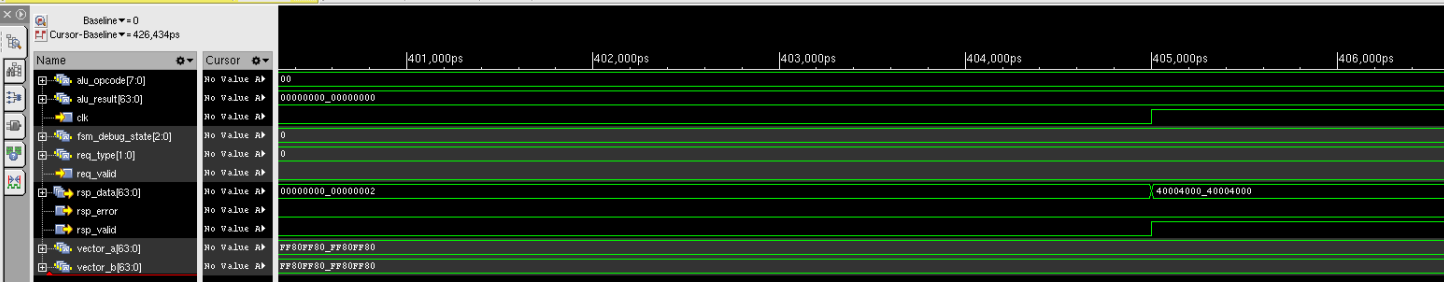
\includegraphics[width=0.96\textwidth]{funcional.png}
\caption{Forma de onda do teste \signal{test_gpu_mul_8bit}. Os vetores de entrada possuem quatro lanes com \signal{FF80} ($-128$) e a resposta de leitura apresenta \signal{4000_4000_4000_4000}, correspondente ao produto \signal{-128 x -128} nas quatro lanes.}
\label{fig:evidencia-e2e}
\end{figure}

\subsection{Cobertura e falhas}

A verificação atingiu 100\% de cobertura funcional, com 44 dos 44 itens
definidos no modelo exercitados. Foram contemplados os tipos de pacote,
opcodes, regiões de endereço dos operandos e do destino, o cruzamento
entre opcode e região de destino, além dos sinais \signal{DONE} e
\signal{rsp_error}. Esse resultado se refere aos cenários definidos no
modelo de cobertura funcional.

Na instância principal da GPU, a cobertura de código atingiu 97,72\%,
com 643 de 658 itens cobertos. Os resultados dos módulos internos foram
medidos separadamente.

\begin{figure}[H]
\centering
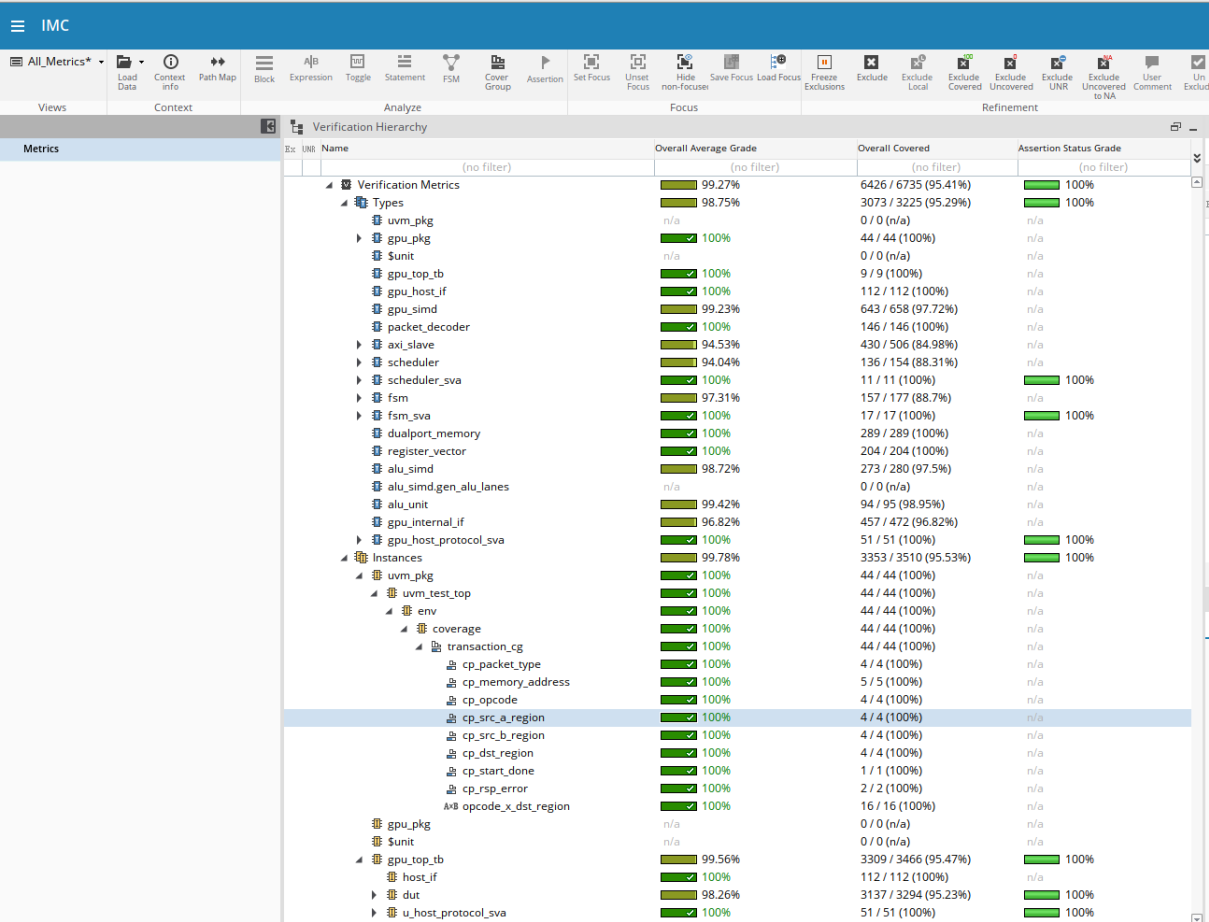
\includegraphics[width=0.96\textwidth]{coverage_imc.png}
\caption{Resumo de cobertura no IMC após a campanha de testes UVM. A instância \signal{gpu_simd} atingiu 643 de 658 itens de código (97,72\%) e o modelo de cobertura funcional atingiu 44 de 44 itens (100\%).}
\label{fig:coverage-summary}
\end{figure}

Durante o desenvolvimento, foi identificada uma falha na inicialização:
o driver podia enviar uma requisição antes de o reset estar definido
como desativado. O driver foi corrigido para aguardar a liberação do
reset antes de transmitir. Outra melhoria foi a ampliação das lanes e
da memória para 16 bits, permitindo preservar o produto completo de
dois operandos signed de 8 bits.

Nas execuções documentadas dos 17 testes UVM, não foram registrados
erros ou falhas fatais.

% =============================================================================
% 6. SINTESE E ANALISE TEMPORAL
% =============================================================================
\section{Síntese e Análise de Timing}

\subsection{Fluxo e resultados de síntese}
O fluxo lê o RTL da mini GPU , elabora o projeto e executa síntese genérica e mapeamento para células padrão. Foram utilizados o canto lento da biblioteca GPDK045, com tensão de 0,9 V e temperatura de 125~$^\circ$C, e as restrições temporais do arquivo SDC. Os resultados a seguir são estimativas da síntese, anteriores à implementação física.

\begin{table}[H]
\centering
\caption{Resumo dos resultados de síntese.}
\label{tab:sintese}
\small
\begin{tabularx}{\textwidth}{lY}
\toprule
\textbf{Métrica} & \textbf{Resultado}\\
\midrule
Ferramenta / versão & Cadence Genus 22.16-s078\_1\\
Biblioteca / tecnologia & GPDK045, \signal{slow_vdd1v0_basicCells.lib}; canto 0,9 V e 125~$^\circ$C\\
Número de células / recursos & 81.398 instâncias: 64.565 combinacionais e 16.833 sequenciais\\
Área estimada & 204.149,034 unidades de área da biblioteca para células\\
Período ou frequência de clock & 20 ns / 50 MHz\\
Restrições relevantes & Incerteza de clock de 1 ns; atrasos de entrada e saída de 1 ns; clock e reset ideais\\
\bottomrule
\end{tabularx}
\end{table}

A memória foi inferida com células padrão, pois o fluxo não utiliza uma IP SRAM compatível, em um projeto industrial é recomendado utilizar uma IP RTL pronta de uma memória para que a ferramenta nãoo a crie utilizando FlipFlops, sua área reportada é 188.340,084 unidades, cerca de 92,26\% da área total de células. A Figura~\ref{fig:esquematico-sintese} apresenta a imagem exportada a partir dessa netlist no Cadence Genus, permitindo visualizar a organização dos blocos e suas conexões. A imagem serve como visão geral; detalhes dos caminhos e das células devem ser examinados na ferramenta.

\begin{figure}[H]
\centering
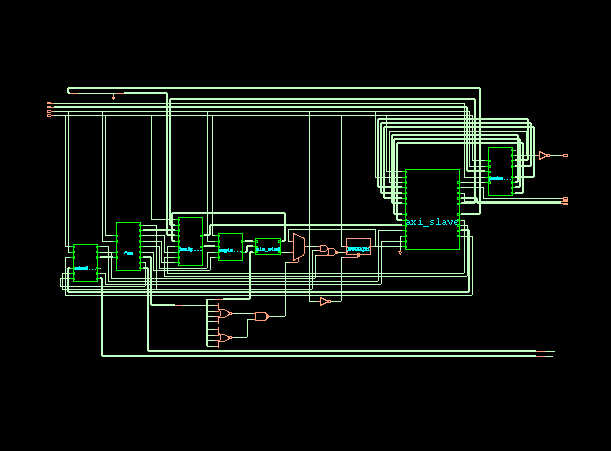
\includegraphics[width=0.8\textwidth]{alu_simd_schematic.png}
\caption{Esquemático exportado da netlist sintetizada no Cadence Genus.}
\label{fig:esquematico-sintese}
\end{figure}

\subsection{Caminho crítico e simulação Gate-Level}
O relatório de síntese identifica um caminho de setup entre um registrador do operando B e um registrador da memória vetorial. O caminho atravessa lógica de divisão de uma lane da ALU e apresenta slack positivo sob a restrição de 20 ns. Esses valores correspondem à análise da netlist sintetizada nas condições e restrições adotadas.

\begin{table}[H]
\centering
\caption{Resumo da análise temporal.}
\label{tab:timing}
\small
\begin{tabularx}{\textwidth}{lY}
\toprule
\textbf{Item} & \textbf{Resultado}\\
\midrule
Ferramenta / relatório & Cadence Genus 22.16-s078\_1; \signal{gpu_simd_timing.rpt}\\
Caminho crítico (origem / destino) & \signal{vector_b_reg[48]/CK} / \signal{mem_reg[254][63]/D}\\
Atraso do caminho de dados & 16,055 ns\\
Slack / resultado do setup & 2,836 ns; restrição atendida\\
Lógica no caminho & Lógica de divisão da lane 3 e seleção para escrita na memória\\
Simulação Gate-Level & Funcional sem SDF: teste registrado como aprovado; simulação com SDF: teste registrado como aprovado\\
Anotação SDF & \signal{gpu_simd.sdf}, valores máximos; 239.898 de 239.914 atrasos de caminho anotados\\
\bottomrule
\end{tabularx}
\end{table}

A análise temporal também foi avaliada por simulação da netlist com anotação dos atrasos do arquivo SDF. Conforme o registro do fluxo, o Cadence Genus gerou o SDF e o Xcelium anotou os valores máximos de atraso na instância da GPU. O testbench executou com período de clock de 20 ns, permitindo observar o comportamento funcional da implementação mapeada sob os atrasos anotados. O registro da execução informa conclusão sem violações temporais.

\begin{figure}[H]
\centering
\fbox{\parbox[c][5cm][c]{0.88\textwidth}{\centering Inserir imagem da simulação temporal da netlist com anotação SDF.\\[0.4em]\small Identificar o clock, os sinais observados e a região temporal correspondente.}}
\caption{Espaço reservado para evidência da simulação temporal com anotação SDF.}
\label{fig:simulacao-sdf}
\end{figure}

% =============================================================================
% 7. LIMITACOES E CONCLUSAO
% =============================================================================
\section{Limitações, Melhorias Futuras e Conclusão}

\subsection{Limitações e melhorias futuras}
A implementação opera com quatro lanes, um único comando de cada vez e quatro operações aritméticas. A interface do host permite escrever operandos de 8 bits, enquanto os resultados internos utilizam lanes de 16 bits; operações sucessivas podem produzir overflow. O modelo de memória foi sintetizado em células padrão, com impacto expressivo na área estimada.

Como trabalhos futuros, podem ser estudados o uso de uma macro SRAM compatível, a otimização do caminho de divisão e a ampliação do conjunto de operações ou da capacidade de processamento. Os resultados de síntese e timing aqui apresentados são anteriores ao posicionamento e roteamento e dependem das restrições e da biblioteca utilizadas.

\subsection{Conclusão}
O projeto integrou memória vetorial, controle e quatro unidades aritméticas em uma mini GPU SIMD descrita em SystemVerilog. Os logs disponíveis registram a execução dos testes UVM sem erros ou falhas fatais, incluindo operações completas e multiplicação de matrizes. O modelo de cobertura funcional atingiu 44 de 44 itens definidos na campanha consolidada.

A síntese sob a restrição de 20 ns apresentou slack positivo de aproximadamente 2,836 ns no caminho crítico reportado. A documentação da simulação temporal também registra conclusão funcional com anotação SDF e sem violações temporais, com os avisos de anotação descritos anteriormente. Esses resultados demonstram o comportamento observado nas condições avaliadas e oferecem uma base para aperfeiçoar a arquitetura e aprofundar sua implementação física.



\end{document}
